\documentclass[]{article}
\usepackage{longtable}
\usepackage{graphicx}
\usepackage{amsmath}
\usepackage{amsfonts}
\usepackage{amssymb}
\usepackage{fullpage}
\usepackage{algorithm}
\usepackage{algorithmic}
\usepackage{bbm}
\usepackage{tikz}
\usepackage{fancyhdr}
\usepackage{array}
\usepackage{longtable}
\usepackage{booktabs}
\usepackage{float}
\usepackage{bbm}
\usepackage{mwe}
\usepackage{minted}
\usepackage{hyperref}
\usepackage{placeins}
\def\marking{CUI//PROPIN}
\allowdisplaybreaks
\setlength{\headheight}{15.2pt}
\setlength{\headsep}{15pt}
\pagestyle{fancy}
\fancyhf{}
\fancyhead{}
\fancyfoot{}
\fancyhead[C]{\marking}
\fancyfoot[C]{\marking}
\fancyfoot[R]{\thepage}
\usetikzlibrary{shapes.geometric, arrows.meta, positioning, fit, backgrounds, calc}

\begin{document}
\begin{center}
\huge Using LLMs to Build Gurobi Models In Record-Breaking Time\\
\normalsize Michael Khalfin\\
\today
\end{center}

\section{Introduction}

Mathematical programming is typically organized around three tasks: modeling, solving, and interpreting results. In the modeling stage, informal requirements and constraints are translated into mathematical objects such as sets, variables, parameters, constraints, and objective functions. Algebraic Modeling Languages (AMLs) provide a software layer for expressing these objects independently of solver-specific details. Pyomo is a widely used AML embedded in Python, allowing users to formulate optimization models with readable Python syntax while retaining access to a broad range of solvers (e.g., CBC, GLPK, IPOPT, CPLEX, or Gurobi) \cite{hart2011pyomo, bynum2021pyomo}. For example, a capacity-constrained supply model can be written in Pyomo as follows:

\begin{minted}{python}
import pyomo.environ as pyo

data = {
    'Plants': ['Plant_A', 'Plant_B'],
    'Markets': ['Market_1', 'Market_2', 'Market_3'],
    'Supply': {'Plant_A': 100, 'Plant_B': 150}
}

def build_pyomo_model(data):
    m = pyo.ConcreteModel()
    m.Plants = pyo.Set(initialize=data['Plants'])
    m.Markets = pyo.Set(initialize=data['Markets'])
    m.x = pyo.Var(m.Plants, m.Markets, domain=pyo.NonNegativeReals)
    m.Supply = pyo.Param(m.Plants, initialize=data['Supply'])

    def supply_rule(m, i):
        return sum(m.x[i, j] for j in m.Markets) <= m.Supply[i]
    m.supply_constr = pyo.Constraint(m.Plants, rule=supply_rule)
    
    def supply_sum(m):
        return sum(m.x[i, j] for i in m.Plants for j in m.Markets)
    m.TotalVolume = pyo.Objective(rule=supply_sum, sense=pyo.maximize)
    
    return m

model = build_pyomo_model(data)
\end{minted}

Following the execution of \texttt{build\_pyomo\_model(data)}, Pyomo constructs a \textit{ConcreteModel}, an in-memory object-oriented representation of the mathematical program. Pyomo sequentially evaluates the provided rules, mapping sets and parameters to decision variables to construct a symbolic algebraic expression tree.

Then, when a user calls a solver, Pyomo must translate its rich expression tree into a format the target solver understands. To handle this translation for Gurobi, Pyomo provides specialized backends. While older pipelines relied on writing intermediate text files (e.g., LP or NL formats) to disk, modern implementations bypass disk I/O entirely using Python bindings. Two of these interfaces are \texttt{gurobi\_direct}, which generates a one-time in-memory Gurobi model, and \texttt{gurobi\_persistent}, which maintains the solver object in memory to facilitate repeated solves without rebuilding. 

However, for large-scale problems with millions of decision variables, Pyomo’s model construction and solver translation steps can become a bottleneck, taking hours or exceeding available memory. Solver-native APIs such as Gurobi’s \texttt{addMVar} and matrix operations avoid much of this overhead by constructing sparse numerical representations directly, but they are typically less readable and harder to modify than AML formulations.

Thus, the standard workflow involves a tradeoff between modeling convenience and construction speed. Recent work on Pyomo \texttt{templatization} reduces model-generation overhead, but it is incompatible with the \texttt{gurobi\_persistent} backend. As a result, the standard workflow in \autoref{fig:diagram1} forces users to choose between faster initial construction and faster iterative re-solving.

\begin{figure}[h]
    \centering
    \resizebox{0.8\textwidth}{!}{%
        \documentclass[tikz, border=25pt]{standalone}
\usetikzlibrary{shapes.geometric, arrows.meta, positioning, fit, backgrounds, calc}

\begin{document}
\begin{tikzpicture}[
    % --- Global Styles ---
    base/.style={draw, thick, align=center, minimum height=0.8cm, minimum width=2.5cm, font=\sffamily},
    data/.style={base, trapezium, trapezium left angle=75, trapezium right angle=105, fill=blue!5},
    source/.style={base, ellipse, fill=blue!5},
    process/.style={base, rectangle, rounded corners, fill=gray!10},
    % Changed the bottleneck to Orange to distinguish it from the Red error state
    bottleneck/.style={process, fill=orange!15, draw=orange!90!black, thick}, 
    decision/.style={base, diamond, fill=yellow!15, aspect=2, inner sep=2pt},
    success/.style={base, ellipse, fill=green!15},
    error/.style={base, rectangle, fill=red!10, draw=red!80!black},
    container/.style={draw, dashed, rounded corners, inner sep=15pt, fill=gray!5},
    arrow/.style={->, >=stealth, thick, color=black!80},
    dashed arrow/.style={->, >=stealth, thick, dashed, color=black!80}
]

    % --- Nodes & Absolute Positioning ---
    
    \node[source] (source) {Source code of\\Pyomo model};
    \node[data, right=1.0cm of source] (data) {User-provided data};

    \node[bottleneck, below=2.5cm of $(source)!0.5!(data)$] (build) {Build Pyomo model};
    \node[process, below=0.8cm of build] (translate) {Translate to Gurobi};
    \node[process, below=0.8cm of translate] (solve) {Solve with Gurobi};

    \node[decision, below=2cm of solve] (feedback) {Result};
    \node[success, below left=1.2cm and 0.8cm of feedback] (sol) {Receive solution};
    \node[error, below right=1.2cm and 1.5cm of feedback] (nosol) {Error: Infeasible\\or unbounded};

    % --- Subgraph Bounding Boxes ---
    % yshift added to ensure the label sits slightly above the dashed line
    \begin{scope}[on background layer]
        \node[container, fit=(source)(data), label={[font=\sffamily\bfseries, xshift=-2mm, yshift=2mm]above left:Writing Code}] (writing) {};
        \node[container, fit=(build)(translate)(solve), label={[font=\sffamily\bfseries, xshift=-2mm, yshift=2mm]above left:Running Code}] (running) {};
        \node[container, fit=(feedback)(sol)(nosol), label={[font=\sffamily\bfseries, xshift=-2mm, yshift=2mm]above left:Output \& Feedback}] (output) {};
    \end{scope}

    % --- Forward Flow Logic ---
    \draw[arrow] (source) -- (build);
    \draw[arrow] (data) -- (build);
    \draw[arrow] (build) -- (translate);
    \draw[arrow] (translate) -- (solve);
    \draw[arrow] (solve) -- (feedback);
    
    \draw[arrow] (feedback) -| node[above, near start, font=\sffamily\small] {Feasible} (sol);
    \draw[arrow] (feedback) -| node[above, near start, font=\sffamily\small] {Infeasible/Unbounded} (nosol);

    % --- Explicit Feedback Loops ---
    
    % Route 1: Out the right, pushed 2.5cm wide. Label moved to the vertical climb (pos=0.25).
    \draw[dashed arrow] (nosol.east) -- ++(2.5,0) |- node[pos=0.25, right, font=\sffamily\small] {Iterate data} (data.east);
    
    % Route 2: Out the bottom, dropped 1cm down, swept 10cm left. Label moved to the vertical climb (pos=0.25).
    \draw[dashed arrow] (nosol.south) -- ++(0,-1.0) -| ++(-10,0) |- node[pos=0.25, left, font=\sffamily\small] {Iterate model} (source.west);

\end{tikzpicture}
\end{document}%
    }
    \caption{The workflow that Pyomo assumes by default.}
    \label{fig:diagram1}
\end{figure}

This workflow has an additional drawback: the user may only discover infeasibility or unboundedness after the Pyomo model has already been built and translated. If the formulation or data must then be revised, the expensive construction process is repeated.

A more efficient workflow is shown in \autoref{fig:diagram2}. The Pyomo formulation remains the canonical, readable specification, but it is immediately \textit{transpiled} into Gurobi-native model-building code rather than instantiated first.\footnote{By transpilation, we mean source-to-source translation: converting Pyomo model-building code into Python code that constructs the corresponding Gurobi model directly.
} This enables faster iteration when the model is infeasible or unbounded. Once feasibility is established, the Pyomo model can be instantiated retroactively to access the benefits of the modeling layer.

\begin{figure}[ht]
    \centering
    \resizebox{0.75\textwidth}{!}{%
        \documentclass[tikz, border=30pt]{standalone}
\usetikzlibrary{shapes.geometric, arrows.meta, positioning, fit, backgrounds, calc}

\begin{document}
\begin{tikzpicture}[
    % --- STYLES ---
    base/.style={draw, thick, align=center, minimum height=0.8cm, minimum width=2.5cm, font=\sffamily},
    data/.style={base, trapezium, trapezium left angle=75, trapezium right angle=105, fill=blue!5},
    source/.style={base, ellipse, fill=blue!5},
    process/.style={base, rectangle, rounded corners, fill=gray!10},
    bottleneck/.style={process, fill=orange!15, draw=orange!90!black, thick},
    decision/.style={base, diamond, fill=yellow!15, aspect=2, inner sep=2pt},
    success/.style={base, ellipse, fill=green!15},
    error/.style={base, rectangle, fill=red!10, draw=red!80!black},
    container/.style={draw, dashed, rounded corners, inner sep=18pt, fill=gray!5},
    arrow/.style={->, >=stealth, thick, color=black!80},
    dashed arrow/.style={->, >=stealth, thick, dashed, color=black!80}
]

    % --- NODES ---
    
    % Phase 1: Writing Code (Loosened vertical spacing to 1.2cm)
    \node[source] (code1) {Code \#1:\\Pyomo model};
    \node[process, below=1.2cm of code1] (transpile) {Run transpilation};
    \node[source, below=1.2cm of transpile] (code2) {Code \#2:\\Direct CVaR Gurobi};
    
    % Pushed data wider to 2.5cm for breathing room
    \node[data, right=2.5cm of code2] (data) {User-provided data};

    % Phase 2: Running Code (Dropped 2.5cm below Phase 1)
    \node[process, below=3.5cm of $(code2)!0.5!(data)$] (build) {Build Gurobi};
    \node[process, below=1.2cm of build] (solve) {Solve with Gurobi};

    % Phase 3: Output & Feedback (Dropped 2.5cm below Phase 2)
    \node[decision, below=2.5cm of solve] (feedback) {Result};
    \node[success, below left=1.5cm and 0.8cm of feedback] (sol) {Receive solution};
    \node[error, below right=1.5cm and 1.5cm of feedback] (nosol) {Error: Infeasible\\ or unbounded};
    
    \node[process, below=1.5cm of sol] (optpyomo) {Build Pyomo\\model retroactively};

    % --- SUBGRAPHS ---
    \begin{scope}[on background layer]
        \node[container, fit=(code1)(transpile)(code2)(data), label={[font=\sffamily\bfseries, xshift=-2mm,yshift=2mm]above left:Writing Code}] (phase1) {};
        \node[container, fit=(build)(solve), label={[font=\sffamily\bfseries, xshift=-2mm, yshift=2mm]above left:Running Code}] (phase2) {};
        \node[container, fit=(feedback)(sol)(nosol)(optpyomo), label={[font=\sffamily\bfseries, xshift=-2mm, yshift=2mm]above left:Output \& Feedback}] (phase3) {};
    \end{scope}

    % --- FORWARD FLOW ---
    \draw[arrow] (code1) -- (transpile);
    \draw[arrow] (transpile) -- (code2);
    
    % V-Funnel into Build
    \draw[arrow] (code2) -- (build);
    \draw[arrow] (data) -- (build);
    
    \draw[arrow] (build) -- (solve);
    \draw[arrow] (solve) -- (feedback);
    
    \draw[arrow] (feedback) -| node[above, near start, font=\sffamily\small] {Feasible} (sol);
    \draw[arrow] (feedback) -| node[above, near start, font=\sffamily\small] {Infeasible/Unbounded} (nosol);

    \draw[arrow] (sol) -- (optpyomo);

    % --- FEEDBACK LOOPS ---
    
    % Right Loop: Iterating Data (Pushed wider to ++(3.5,0) so it stays well clear of the boxes)
    \draw[dashed arrow] (nosol.east) -- ++(3.5,0) |- node[pos=0.25, right, font=\sffamily\small] {Iterate data} (data.east);
    
    % Left Loop: Iterating Pyomo Model 
    % Dropped lower to ++(0,-2.5) to cleanly sweep under the Optional Pyomo block, and swept wider left to ++(-11,0)
    \draw[dashed arrow] (nosol.south) -- ++(0,-3.5) -| ++(-11,0) |- node[pos=0.25, left, font=\sffamily\small] {Iterate Pyomo model} (code1.west);

\end{tikzpicture}
\end{document}%
    }
    \caption{The Pyomo-to-Gurobi workflow developed in this paper, which preserves Pyomo as the canonical specification while enabling direct Gurobi-native model construction. 
    % (We can have our cake and eat it too.)
    }
    \label{fig:diagram2}
\end{figure}
\clearpage

The central idea of this paper is that a frontier large-language model (LLM), used through an agentic coding workflow, can generate and refine a deterministic Python transpiler that converts human-readable Pyomo formulations into Gurobi-native model-building code. As shown in \autoref{fig:diagram3}, the stochastic component is confined to development of the transpiler. Once generated, the transpiler is an ordinary Python artifact: deterministic in execution, inspectable, testable, benchmarkable, and repairable.

\begin{figure}[ht]
    \centering
    \resizebox{0.75\textwidth}{!}{%
        \begin{tikzpicture}[
    % --- STYLES ---
    base/.style={draw, thick, align=center, minimum height=1cm, minimum width=3cm, font=\sffamily},
    data/.style={base, trapezium, trapezium left angle=75, trapezium right angle=105, fill=blue!5},
    source/.style={base, ellipse, fill=blue!5},
    process/.style={base, rectangle, rounded corners, fill=gray!10},
    agent/.style={process, fill=purple!15, draw=purple!80!black, thick}, 
    memory/.style={process, shape=cylinder, aspect=0.25, draw, shape border rotate=90, fill=gray!20, minimum height=1.5cm}, 
    script/.style={process, fill=blue!10, draw=blue!80!black, thick, minimum width=4cm}, 
    decision/.style={base, diamond, fill=yellow!15, aspect=2, inner sep=2pt},
    success/.style={base, rectangle, rounded corners, fill=green!15, draw=green!60!black, thick},
    container/.style={draw, dashed, rounded corners, inner sep=20pt, fill=gray!5},
    arrow/.style={->, >=stealth, thick, color=black!80},
    dashed arrow/.style={->, >=stealth, thick, dashed, color=black!80}
]

    % ==========================================
    % RUNTIME TRANSPILATION (Bottom Box)
    % ==========================================
    
    % 1. Core Pipeline
    \node[script] (transpiler) {Deterministic Python\\Transpiler Script};
    \node[source, left=2.5cm of transpiler] (code1) {Code \#1:\\New Pyomo instance};
    \node[source, right=2.5cm of transpiler] (code2) {Code \#2:\\Gurobi-native code};
    
    % 2. Testing Layer
    \node[decision, below=2.5cm of transpiler] (test) {Execute\\Test Suite};
    \node[data] at (code1 |- test) (data) {User-provided data};
    
    % 3. Deployment
    \node[success, below=2cm of test] (deploy) {Use the code};

    % Runtime Arrows
    \draw[arrow] (code1) -- node[above, font=\sffamily\small] {Processed by} (transpiler);
    \draw[arrow] (transpiler) -- node[above, font=\sffamily\small] {Outputs} (code2);
    
    \draw[arrow] (code1.south) -- (test.north west);
    \draw[arrow] (code2.south) -- (test.north east);
    \draw[arrow] (data.east) -- (test.west);
    
    \draw[arrow] (test.south) -- node[right, font=\sffamily\small] {Pass} (deploy.north);

    % ==========================================
    % AGENTIC GENERATION (Top Box)
    % ==========================================
    
    \node[agent, above=3.5cm of transpiler] (agent) {LLM Agent};
    \node[memory] at (code1 |- agent) (repo) {Examples/\\Repository};
    
    % Agentic Arrows
    \draw[dashed arrow] (agent.south) -- node[right, font=\sffamily\small] {Generates / Refactors} (transpiler.north);
    \draw[arrow] (repo.east) -- (agent.west);

    % ==========================================
    % WIDE FEEDBACK LOOPS
    % ==========================================
    
    % Fail Loop: Out the right side of the test suite decision box
    \draw[dashed arrow] (test.east) -- ++(9,0) |- node[pos=0.25, right, font=\sffamily\small, align=center] {Fail:\\Send output\\to agent} (agent.east);
    
    % Save to Repo Loop: Creates a junction node on the "Pass" line to trigger the save action
    % Sweeps 7cm to the left, clear of Code 1 and Data, right into the repository
    \draw[dashed arrow] ($(test.south)!0.5!(deploy.north)$) -| ++(-11,0) |- node[pos=0.25, left, font=\sffamily\small, align=center] {Vetted instance \& code\\saved as dynamic tests\\for the agent} (repo.west);

    % ==========================================
    % BOUNDING BOXES
    % ==========================================
    \begin{scope}[on background layer]
        \node[container, fit=(agent)(repo), label={[font=\sffamily\bfseries, yshift=2mm]above left:Agentic Generation (Stochastic, resource-heavy)}] (phase1) {};
        
        \node[container, fit=(code1)(transpiler)(code2)(data)(test)(deploy), label={[font=\sffamily\bfseries, yshift=2mm]above left:Runtime Transpilation (Deterministic, instantaneous)}] (phase2) {};
    \end{scope}

\end{tikzpicture}%
    }
    \caption{Development and verification of the transpiler using an agentic loop. Note that the 4 process nodes are the same as in \autoref{fig:diagram2}.}
    \label{fig:diagram3}
\end{figure}

Its outputs are vetted by differential testing. For a given formulation, both the original Pyomo code and the transpiled Gurobi-native code are executed on the same data, and the resulting solver-level model structures are compared. Because the data is an explicit input, this validation is computationally inexpensive: we can repeatedly test on truncated datasets that preserve the full problem's indexing structure while keeping Pyomo's instantiation quick. If the two implementations construct identical models across multiple reduced instances, it becomes highly unlikely that the transpiler is merely coincidentally correct. The same deterministic code can then be run at full scale.

This approach provides a different trust model from much of the recent literature on LLMs for optimization. Rather than treating the LLM as a black-box optimizer or an oracle for formulation quality, we deploy it to produce an intermediate software artifact whose behavior can be validated and iteratively repaired. Failed tests are returned to the agent, while passing cases are retained as regression tests. Although we focus on Pyomo-to-Gurobi transpilation, the methodology generalizes across the modeling ecosystem: LLM-assisted transpilers can translate between any AMLs, solver APIs, or optimization transformations. More broadly, this pattern of data-parametric validation applies whenever a trusted reference implementation exists and is highly dependent on input data. By validating equivalence on reduced instances, developers can confidently deploy deterministic, agent-generated code at scale.

To demonstrate the efficacy of this approach, we preview the build times for three canonical models in \autoref{tab:supply-demand}, \autoref{tab:network-flow}, and \autoref{tab:bom}. These tables compare standard Pyomo, Pyomo-templatization, an early transpiler version using \texttt{gurobipy-pandas}, and our current transpiler utilizing COO arrays and \texttt{addMVar}. Section~\ref{sec:results} details these canonical problems, alongside an in-depth case study of a large-scale epidemic model—the specific use case that motivated this framework.

\begin{table}[H]
\centering
\caption{Build times for the Supply-Demand problem.
\texttt{gurobipy-pandas} denotes Claude Code's initial generated implementation using the \texttt{gurobipy-pandas} library; COO+MVar denotes the current Gurobi-native implementation using sparse COO matrices and \texttt{MVar}.}
\label{tab:supply-demand}
\begin{tabular}{lrrrrr}
\toprule
Size & Variables & Pyomo & Pyomo+Template & gurobipy-pandas & COO+MVar \\
\midrule
\(2300^2\) & 5,290,000  & 0.823 & 0.206 & 0.376 & 0.051 \\
\(3300^2\) & 10,890,000 & 1.955 & 0.410 & 0.766 & 0.107 \\
\(4700^2\) & 22,090,000 & 6.328 & 0.900 & 1.605 & 0.227 \\
\(6500^2\) & 42,250,000 & 70.699 & 2.241 & 3.188 & 0.506 \\
\(9000^2\) & 81,000,000 & TIMEOUT & 9.285 & 6.758 & 1.221 \\
\bottomrule
\end{tabular}
\end{table}

\begin{table}[H]
\centering
\caption{Build times for the Network Flow problem.}
\label{tab:network-flow}
\begin{tabular}{lrrrrr}
\toprule
Size & Variables & Pyomo & Pyomo+Template & gurobipy-pandas & COO+MVar \\
\midrule
\(n=5000,k=175\)  & 5,250,000  & 1.142 & 0.302 & 0.470 & 0.087 \\
\(n=7500,k=225\)  & 10,125,000 & 2.340 & 0.602 & 0.900 & 0.166 \\
\(n=11000,k=285\) & 18,810,000 & 8.707 & 1.272 & 1.741 & 0.322 \\
\(n=16000,k=360\) & 34,560,000 & 105.128 & 2.886 & 3.581 & 0.701 \\
\(n=22000,k=430\) & 56,760,000 & TIMEOUT & 5.849 & 6.627 & 1.361 \\
\bottomrule
\end{tabular}
\end{table}

\begin{table}[H]
\centering
\caption{Build times for the Bill-of-Materials problem.}
\label{tab:bom}
\begin{tabular}{lrrrrr}
\toprule
Size & Variables & Pyomo & Pyomo+Template & gurobipy-pandas & COO+MVar \\
\midrule
\(p=10k,c=20k,t=80\)  & 2,400,000  & 0.774 & 0.172 & 0.176 & 0.053 \\
\(p=15k,c=30k,t=100\) & 4,500,000  & 1.479 & 0.337 & 0.328 & 0.098 \\
\(p=22k,c=44k,t=120\) & 7,920,000  & 2.948 & 0.635 & 0.594 & 0.177 \\
\(p=32k,c=64k,t=150\) & 14,400,000 & 15.080 & 2.439 & 1.181 & 0.351 \\
\(p=45k,c=90k,t=180\) & 24,300,000 & 116.675 & 2.942 & 2.241 & 0.619 \\
\bottomrule
\end{tabular}
\end{table}

\paragraph{Contributions} In summary, this paper makes the following contributions:
\begin{enumerate}
    \item \textbf{Agent-Generated Transpilation}: We demonstrate that an agentic LLM workflow can successfully construct a deterministic Python transpiler. This artifact bridges the abstraction gap, automatically translating human-readable Pyomo models into Gurobi-native C-API structures to achieve massive build-time speedups.
    \item \textbf{Data-Parametric Verification}: We formalize a differential testing suite that leverages reduced datasets to strictly verify the transpiler's output against the original Pyomo model. This data-truncated validation mirrors the rigorous vetting workflows standard in national laboratory and industrial settings, showing algorithmic correctness before scaling to full production instances.
    \item \textbf{A Generalized Software Methodology}: We establish that pairing agent-driven generation with validation provides a blueprint for bridging structural gaps. When a translation is required between any two rigorous representations, an agent can attempt to synthesize the missing bridge. The prerequisite is an independent verification mechanism—whether through data-parametric testing or formal software provers like Rocq—making this methodology applicable across a vast array of computational and engineering domains.
\end{enumerate}

\section{Background: LLMs in OR and Code Generation}

\paragraph{LLMs in OR.} Recent papers increasingly use LLMs to formulate mixed-integer linear programming problems directly from natural language descriptions. For example, the NL4Opt competition challenged participants to generate intermediate representations of linear programs from text for use by commercial solvers \cite{ramamonjison2023nl4opt}, building on earlier efforts to simplify the OR modeling experience \cite{ramamonjison2022augmenting}. This has spurred the creation of dedicated optimization benchmarks \cite{yang2025optibench} and a variety of generative approaches. Multi-agent frameworks such as OptiMUS \cite{ahmaditeshnizi2024optimus-2, ahmaditeshnizi2024optimus-1} and others \cite{xiao2024chain} parse complex natural language descriptions into programmatic constraints and objectives, while recent training-free architectures like SolverLLM leverage test-time search algorithms to iteratively guess and refine formulations \cite{li2026solverllm}. Due to elevated computational costs and privacy concerns of frontier models, efforts like \cite{huang2025orlm} have even trained open-source LLMs specifically for this task. A related stream of research deploys LLMs as interactive AI assistants to query model states \cite{li2023large} and debug infeasible Pyomo formulations \cite{chen2024diagnosing}. These tools are primarily aimed at making optimization modeling accessible to non-experts, either by generating formulations from natural language or by supporting conversational interaction with existing models. Our focus is different. We assume that the algebraic model itself remains the rigorous source of truth, and ask how developers can preserve that exact, inspectable representation while making model construction and solver interaction substantially faster.

Beyond formulation, recent work has even applied LLMs to the algorithmic solving phase of MILPs \cite{iklassov2024self, sun2026co, ye2025large}, including heuristic tasks such as cold-start cutting plane configuration \cite{lawless2025llms}. These methods operate downstream of model construction and are therefore complementary to our framework.

\paragraph{LLMs in Code Generation and Transpilation.} A more direct antecedent to our work is LLM-assisted code transpilation: translating code from one language or representation into another. Recent systems have used LLMs for verified lifting into domain-specific languages \cite{bhatia2024verified}, C-to-Rust migration with iterative repair \cite{farrukh2026safetrans}, transpilation combined with program repair \cite{ramos2024batfix}, and cross-language translation among general-purpose languages such as C, C++, Java, and Python \cite{rai2024cross}. These works highlight both the promise and the risk of LLM-generated code: the generated artifact can often be useful, but must be checked, repaired, or otherwise validated.

Our work follows this line of thinking in an optimization modeling context, using Pyomo as the reference implementation and Gurobi-native code as the transpilation target. 

Our implementation uses Claude Code (powered by Claude Opus 4.8) as an agentic coding environment. Recent reports suggest that such systems can be effective on compiler-scale software projects. Notably, parallel Claude agents successfully authored a Rust-based C compiler through iterative task selection, testing, and repair \cite{carlini2026compiler}. These long-running agentic workflows excel when grounded in deterministic tests, compact feedback, and rich repository context. In our framework, this context explicitly includes the source code of the Pyomo library itself, which embodies substantial prior work in algebraic modeling. Providing the agent with direct access to Pyomo's internal architecture makes the task more constrained than open-ended generation settings, where the model must invent premises or process steps from ambiguous information \cite{zahavyposition}. Here, the source program already exists, the target API is well defined, and the desired behavior can be checked against Pyomo. The LLM constructs a compiler-like translation path from one exact representation to another.

Beyond benchmarks and context, successful agentic generation relies on human-in-the-loop planning. Anthropic's analysis of Claude Code usage indicates that domain expertise remains critical for specifying architectural objectives and recognizing correct outcomes \cite{anthropic2026expertise}. As detailed in Section~\ref{sec:methods}, our workflow relies on active human prompting to direct the agentic loop. We provide the requisite optimization expertise—both by authoring the canonical Pyomo source models and by continually guiding the agent's objectives—while Claude Code executes the software engineering required to construct and refine the transpiler.

\section{Methods: Agentic Generation of the Transpiler}
\label{sec:methods}

Section~\ref{sec:methods-env} describes the agent's environment and context; Section~\ref{sec:methods-decomp}, the decomposition of the task and the prompting strategy. Section~\ref{sec:methods-verify} presents the differential-testing framework that certifies each transpiled model, and Section~\ref{sec:methods-transpiler} describes the transpiler it produced.

\subsection{The Agentic Environment and Context}
\label{sec:methods-env}

The transpiler was engineered within an agentic coding environment primarily driven by Claude Opus~4.8, supplemented by Claude Sonnet~4.6 for targeted refactoring and Claude Fable~5 for code reviews. The agent operates inside the project repository through an autonomous read--edit--run--observe cycle: it reads a file, changes it, executes the result, and inspects the output before the next step. To isolate development during trial-and-error phases, the agent operates within a dedicated Git branch, generating code changes locally and proposing formal software patches only when a stable iteration of the transpiler passes all verification checks. \autoref{tab:agent-env} inventories what the agent could read and do.

\begin{table}[ht]
\centering
\caption{The resources available to the agent in the repository.}
\label{tab:agent-env}
\small
\begin{tabular}{@{}p{0.23\textwidth}p{0.71\textwidth}@{}}
\toprule
\textbf{Reference Libaries} & Pyomo source code files (local environment installation); \texttt{gurobipy-pandas} and \texttt{gurobipy} API documentation (read-only) \\
\textbf{Repository Artifacts} & Transpiler source code; $21$ canonical Pyomo models serving as the differential and regression testing library (read/write) \\
\textbf{Testing \& Performance} & Differential testing suite; computational benchmarking scripts (read/write) \\
\textbf{Actions} & Workspace regex search; read files; edit source; run shell commands and Python scripts (build, solve, test, benchmark); read output and error logs; persistent cross-session state memory \\
\bottomrule
\end{tabular}
\end{table}

One property of this setup separates it from open-ended code generation: both endpoints of the translation path are fully specified \emph{in the workspace}. The source language is Pyomo's own source code, and the target is bounded by the Gurobi API. The agent translates between two exact representations rather than inferring either of them. Because the Pyomo reference and the generated candidate share the repository, every emitted model can be executed and compared against ground truth on the spot (Section~\ref{sec:methods-verify}). The human contributes the domain-specific optimization models and architectural objectives, while the agent contributes the underlying software engineering \cite{anthropic2026expertise, carlini2026compiler}.

\subsection{Task Decomposition and Prompting}
\label{sec:methods-decomp}

% [To be written: decomposition of the translation task into agent-sized
%  subtasks, the prompting strategy that drove the agentic loop, and the
%  human-in-the-loop guidance that accompanied it.]

\subsection{Verification by Differential Testing}
\label{sec:methods-verify}

The transpiler is trusted only because each model it emits is checked against Pyomo. Establishing that two Gurobi models coincide is subtler than a field-by-field comparison: the pipelines emit variables and constraints in different orders and under different names, so equality holds only up to a permutation of rows and columns. Cast each model as the bipartite incidence graph between its variables and its constraints---an edge, weighted by the coefficient $a_{uv}$, wherever variable $v$ appears in constraint $u$---and the two models agree exactly when these labelled graphs are isomorphic.

We test this isomorphism efficiently by computing a permutation-invariant \emph{signature} in two layers (\autoref{tab:signature}). The first layer deals with both nodes and edges, but ignores how they connect. It consists of order-independent multisets, such as global counts, coefficient values, variable bounds, and right-hand sides. A mismatch at this layer instantly flags a defect and isolates the specific parameter that the transpiler mishandled. However, these summaries cannot detect incidence errors, such as a correct coefficient being assigned to the wrong variable.

To capture this incidence structure, the second layer applies \emph{color refinement} (the 1-dimensional Weisfeiler-Leman algorithm). Each node is initialized with a ``color'' (a hash) encoding its intrinsic properties: a variable's bounds, type, and objective coefficient; or a constraint's sense and right-hand side. In each iteration $t$, every node is recolored by hashing its current color with the multiset of its neighbors' colors and the connecting edge weights (the constraint coefficients $a_{uv}$):
\begin{equation}
c_{t+1}(v) \;=\; \mathrm{hash}\!\Big( c_t(v),\; \big\{\, (c_t(u),\, a_{uv}) : u \in N(v) \,\big\} \Big),
\label{eq:wl}
\end{equation}
Here, $\operatorname{hash}(\cdot)$ denotes a deterministic, collision-resistant mapping (e.g., SHA-256) that assigns a uniquely identifiable integer to each distinct input state. The process repeats until the color distribution stabilizes. Structurally interchangeable nodes converge to a common color, and the final histogram of colors perfectly characterizes the incidence graph. Two models are declared structurally equivalent only if both layers of their signatures match exactly.

\begin{table}[ht]
\centering
\caption{The two layers of the structural signature and the discrepancy each detects. Every component is invariant to relabeling of variables and constraints.}
\label{tab:signature}
\small
\begin{tabular}{@{}p{0.42\textwidth}p{0.52\textwidth}@{}}
\toprule
\textbf{Signature component} & \textbf{Discrepancy it detects} \\
\midrule
Counts $(V, C, \mathrm{nnz})$ & missing or extra variable, constraint, or term \\
Coefficient multiset & wrong constraint coefficient \\
Right-hand-side multiset & wrong right-hand side \\
Objective-coefficient multiset & wrong objective weight \\
Bound/type multiset $(\ell, u, \tau)$ & wrong variable bound or domain \\
\midrule
Colour-refinement histogram, Eq.~\eqref{eq:wl} & wrong incidence: which variables enter which constraints \\
\bottomrule
\end{tabular}
\end{table}

Two conventions are folded out so that equivalent models are not flagged. An equality row and its negation state the same constraint, so each equality is encoded by the \emph{unordered} pair of its positive- and negative-coefficient sides, which negation merely swaps. And a right-hand side of $-0.0$, which the transpiler's arithmetic can yield where Pyomo yields $0.0$, is normalized before hashing.

Because the data is an argument to the model function, the check runs on \emph{reduced} instances that retain the index structure but shrink every set, so Pyomo instantiates them in milliseconds. We test each benchmark model at several sizes and three seeds---thirty instances---together with twenty-one formulations that each isolate one modeling feature. As the transpiler is deterministic, code certified on these instances is exactly the code that runs at scale.

A check that cannot fail certifies nothing, so we confirm the signature detects deliberate corruptions of a correct model (\autoref{tab:controls}); the count-only comparison misses three of the four. This sensitivity is what exposed the omitted upper bound of Section~\ref{sec:results-verify}, which left every count unchanged. In the loop, a failing signature names the differing component---localized feedback for repair---and each newly passing model is retained as a regression, so the certified class grows monotonically.

\begin{table}[ht]
\centering
\caption{Negative controls. Each corruption of a correct model must change the signature; comparing variable and constraint counts alone---the naive check---misses three of the four.}
\label{tab:controls}
\small
\begin{tabular}{@{}p{0.40\textwidth}p{0.36\textwidth}p{0.15\textwidth}@{}}
\toprule
\textbf{Corruption} & \textbf{First flagged by} & \textbf{Counts alone?} \\
\midrule
Remove a constraint & counts $(C, \mathrm{nnz})$ & yes \\
Tighten a variable bound & bound multiset & no \\
Perturb one coefficient & coefficient multiset, colours & no \\
Alter an objective coefficient & objective multiset & no \\
\bottomrule
\end{tabular}
\end{table}

\subsection{The Transpiler}
\label{sec:methods-transpiler}

The transpiler is a deterministic compiler from a Pyomo model function to the source of an equivalent Gurobi builder. It never executes Pyomo: it reads the function as text, so none of Pyomo's construction cost is paid. Its stages mirror a compiler---parse, classify, reconcile indices, generate (\autoref{fig:pipeline})---and only classification embeds modeling knowledge.

\begin{figure}[ht]
\centering
\resizebox{\textwidth}{!}{%
\begin{tikzpicture}[
  box/.style={draw, rounded corners, align=center, minimum height=12mm, inner sep=2.4mm, fill=black!4},
  arr/.style={-{Latex[length=2.4mm]}, thick}]
\node[box] (src) {Pyomo model\\function (text)};
\node[box, right=20mm of src] (dec) {declarations:\\sets, params,\\vars, constraints};
\node[box, right=20mm of dec] (pat) {constraints tagged\\by shape,\\index registry};
\node[box, right=20mm of pat] (gen) {\texttt{build\_vectorized\_model}\\\texttt{update\_vectorized\_model}};
\draw[arr] (src) -- node[above, font=\scriptsize]{parse (AST)} (dec);
\draw[arr] (dec) -- node[above, font=\scriptsize]{classify} (pat);
\draw[arr] (pat) -- node[above, font=\scriptsize]{generate} (gen);
\end{tikzpicture}}
\caption{The transpiler as a compiler. Only the \emph{classify} stage embeds modeling knowledge---the catalog of constraint shapes in \autoref{tab:patterns}; parsing and code generation are mechanical. The output is Gurobi-native source, never an instantiated Pyomo model.}
\label{fig:pipeline}
\end{figure}

\paragraph{Where the work runs.} The speedup is a matter of \emph{where} construction happens, not its asymptotic order. Let $V$, $C$, and $N$ denote the numbers of variables, constraints, and nonzero coefficients. Standard Pyomo evaluates each rule into an expression tree and allocates one Python object per variable and per constraint---$\Theta(V + C + N)$ interpreted allocations before the model reaches the solver---and the large per-object constant, with its attendant memory traffic, is what makes construction superlinear in practice (Section~\ref{sec:results-timing}). Templatization removes the per-row trees but still allocates the $\Theta(V)$ variable objects. The transpiler allocates none: it emits a fixed number of library calls, independent of instance size, and performs the $\Theta(N)$ assembly of the constraint matrix in compiled array code through pandas and SciPy (\autoref{tab:complexity}). Its cost tracks nonzeros in compiled code rather than components in interpreted code.

\begin{table}[ht]
\centering
\caption{Construction cost for a model with $V$ variables, $C$ constraints, and $N$ nonzero coefficients. The pipelines share the $\Theta(N)$ order but differ in whether that work runs as interpreted object allocation or compiled array code, and in how many size-dependent Python-level operations they issue.}
\label{tab:complexity}
\small
\begin{tabular}{@{}p{0.20\textwidth}p{0.18\textwidth}p{0.19\textwidth}p{0.13\textwidth}p{0.11\textwidth}@{}}
\toprule
\textbf{Pipeline} & \textbf{Intermediate form} & \textbf{Python object allocations} & \textbf{Where $\Theta(N)$ runs} & \textbf{In-place re-solve} \\
\midrule
Pyomo (\texttt{persistent}) & expression tree per constraint & $\Theta(V + C + N)$ & interpreted & yes \\
Pyomo + templatization & one template per block & $\Theta(V)$ & interpreted & no \\
Transpiler (COO+MVar) & sparse COO arrays & $O(1)$ in $V, C$ & compiled & yes \\
\bottomrule
\end{tabular}
\end{table}

\paragraph{From a rule to a matrix.} The assembly is a relational join. Take the supply constraint $\sum_{j \in J} x_{ij} \le s_i$. Number the variables by a bijection $\gamma:(i,j)\mapsto\{0,\dots,|I||J|-1\}$ and the rows by $\rho:i\mapsto\{0,\dots,|I|-1\}$; the block is $A\in\{0,1\}^{|I|\times|I||J|}$ with $A_{\rho(i),\,\gamma(i,j)}=1$. From a table of variable columns $\{(i,j,\gamma(i,j))\}$ and a table of constraint rows $\{(i,\rho(i))\}$, an equi-join on the shared index $i$ yields exactly the nonzero coordinates $(\rho(i),\gamma(i,j))$; these become a sparse matrix passed to Gurobi as \texttt{addMConstr}$(A,\,x,\,{\le},\,s)$. A weighted sum $\sum_j w_{ij}x_{ij}$ simply carries $w_{ij}$ as the join's coefficient column in place of $1$.

Each shape the transpiler recognizes is one such recipe (\autoref{tab:patterns}): a join that produces the nonzero coordinates, a coefficient column, and a sparse assembly. The capacity, flow-conservation, and bill-of-materials constraints of Section~\ref{sec:results-problems} are all instances.

\begin{table}[ht]
\centering
\caption{Representative constraint shapes and the sparse-assembly recipe each compiles to. The relation is $\le$, $=$, or $\ge$; the objective, when present, is assembled the same way as a single row.}
\label{tab:patterns}
\small
\begin{tabular}{@{}p{0.17\textwidth}p{0.33\textwidth}p{0.44\textwidth}@{}}
\toprule
\textbf{Shape} & \textbf{Algebraic form} & \textbf{Assembly} \\
\midrule
Grouped sum & $\sum_{j} w_{ij}\,x_{ij} \le b_i$ & join variable table with row table on the shared index; coefficient $w_{ij}$ (or $1$) \\
Flow balance & $\sum_{\delta^+(n)} x - \sum_{\delta^-(n)} x = b_n$ & two joins on the out/in arc sets, coefficients $+1/-1$, concatenated \\
Cross-dimensional & $z_{ct} = \sum_{p\in P(c)} a_{pc}\,y_{pt}$ & join $a$ with $y$ on $p$, then with the row table on $(c,t)$; coefficient $a_{pc}$; the $z$ term contributes $-I$ \\
Direct bound & $x_i \le b_i$ & one nonzero per row (identity-like) \\
Linear combination & $\sum_i (\alpha x_i + \beta y_i) \le b$ & one block per variable term, each with its own coefficient \\
\bottomrule
\end{tabular}
\end{table}

\paragraph{Build and update.} The generated module exposes two functions. \texttt{build\_vectorized\_model} constructs the model; \texttt{update\_vectorized\_model} overwrites the right-hand sides and objective coefficients of an existing model in $\Theta(N)$ without touching its structure, so a model is re-solved under revised data at negligible cost. This is the re-solve loop of \autoref{fig:diagram2}, and the capability templatization forfeits through its incompatibility with the persistent backend.

The transpiler is deliberately restricted to linear models whose constraints fall within the catalog and that observe a few authoring conventions---index arithmetic precomputed into sets, no data-dependent branching inside a rule. The restriction is what keeps the pattern match sound and the output checkable; the catalog itself grew example by example, each new shape locked in by a regression (Section~\ref{sec:methods-verify}).

\section{Computational Results}
\label{sec:results}

We evaluate the transpiler along two independent axes. Section~\ref{sec:results-problems} introduces three benchmark formulations that exercise the range of indexing structures the transpiler must handle. Section~\ref{sec:results-verify} establishes correctness, certifying that each transpiled model is structurally identical to the model Pyomo builds across many reduced instances. Section~\ref{sec:results-timing} quantifies the construction-time advantage of the transpiled workflow over Pyomo's native backends. Finally, Section~\ref{sec:results-epidemic} applies the framework to the large-scale epidemic model that originally motivated it.

\subsection{Benchmark Models}
\label{sec:results-problems}

We use three parameterized model families. Each is a feasibility formulation---a set of decision variables and constraints without an objective---since our concern is the cost of \emph{constructing} the model rather than solving it. Each family is specified once as a Pyomo model-building function and paired with a data generator that emits instances of arbitrary size from a fixed random seed, so that the same specification produces both the small instances used for verification and the large instances used for timing.

\paragraph{Supply--Demand.} Given a set of sources $I$ and destinations $J$, with supply $s_i \ge 0$ available at each source and demand $d_j \ge 0$ required at each destination, the decision variables $x_{ij} \ge 0$ denote the quantity shipped from $i$ to $j$. A feasible shipping plan satisfies
\[
\sum_{j \in J} x_{ij} \le s_i \quad \forall i \in I, \qquad
\sum_{i \in I} x_{ij} \ge d_j \quad \forall j \in J, \qquad
x_{ij} \ge 0 .
\]
An instance has $|I| \times |J|$ variables.

\paragraph{Multi-Commodity Network Flow.} On a directed graph with nodes $N$ and arcs $E \subseteq N \times N$, a set of commodities $K$ must be routed simultaneously. For each node $n$, let $\delta^{+}(n)$ and $\delta^{-}(n)$ denote its outgoing and incoming arcs. Each arc $(i,j)$ has capacity $u_{ij} \ge 0$ shared across commodities, and $b_{nk}$ is the net flow of commodity $k$ required at node $n$. The variables $x_{ijk} \ge 0$ carry commodity $k$ on arc $(i,j)$, and a feasible routing satisfies
\[
\sum_{k \in K} x_{ijk} \le u_{ij} \quad \forall (i,j) \in E, \qquad
\sum_{j \in \delta^{+}(n)} x_{njk} \;-\; \sum_{i \in \delta^{-}(n)} x_{ink} = b_{nk} \quad \forall n \in N,\, k \in K,
\]
with $x_{ijk} \ge 0$. The adjacency sets $\delta^{+}(\cdot)$ and $\delta^{-}(\cdot)$ are precomputed and supplied as indexed sets.

\paragraph{Bill-of-Materials.} A production model links product builds to component purchases across periods. Over products $P$, components $C$, and periods $T$, let $P(c) \subseteq P$ be the products that use component $c$, let $a_{pc} \ge 0$ be the amount of $c$ consumed per unit of $p$, and let $U_{pt} \ge 0$ be the capacity for building $p$ in period $t$. The variables $y_{pt} \ge 0$ and $z_{ct} \ge 0$ denote the amount of product $p$ built and component $c$ bought in period $t$. A feasible plan satisfies
\[
y_{pt} \le U_{pt} \quad \forall p,\, t, \qquad
z_{ct} = \sum_{p \in P(c)} a_{pc}\, y_{pt} \quad \forall c \in C,\, t \in T, \qquad
y_{pt} \ge 0,\; z_{ct} \ge 0 .
\]
The coupling parameter $a_{pc}$ is stored over the product--component pairs that actually occur, rather than over the dense grid $P \times C$; as Section~\ref{sec:results-timing} shows, expressing this sparsity in the index structure is decisive for construction speed.

\subsection{Verification of Equivalence}
\label{sec:results-verify}

Before comparing construction times, we confirm that the transpiled code and the Pyomo reference build the same model. Using the differential-testing procedure of Section~\ref{sec:methods-verify}, we compare the two solver-level models on many small instances drawn from the same specifications as the benchmarks. Because the data is an explicit argument and the reduced instances retain the indexing structure of the full model, Pyomo instantiation stays inexpensive and equivalence can be checked broadly rather than on a single case. Across $30$ reduced instances of the three benchmark models---each at several sizes and three random seeds---and $21$ additional formulations that isolate individual modeling features, every transpiled model is structurally identical to its Pyomo reference. The same procedure surfaced a genuine defect during development: on a formulation whose variables carried explicit interval bounds, the transpiler had dropped the upper bound, leaving the model dimensions unchanged but enlarging its feasible region. The discrepancy was repaired and retained as a regression test. Having established equivalence, we turn to construction time.

\subsection{Build-Time Performance}
\label{sec:results-timing}

Having established equivalence, we measure construction time. We compare four pipelines, all derived from the same Pyomo model-building function: standard Pyomo through \texttt{gurobi\_persistent}; Pyomo with constraint and objective templatization compiled through Gurobi's matrix interface (\texttt{gurobi\_direct}); the transpiler's initial \texttt{gurobipy-pandas} output; and its current output built from sparse coordinate-format matrices via \texttt{addMVar} and \texttt{addMConstr} (COO+MVar). Reported times measure model construction only and exclude the solve. Each build is timed with the cyclic garbage collector disabled and a full collection forced beforehand, so that garbage-collection activity during the construction of the many-object Pyomo models does not distort the measurement. We impose a construction budget of $25$ minutes per instance: once a pipeline exceeds this budget at a given size, larger instances of the same family are not attempted and are reported as timeouts. \autoref{tab:supply-demand}, \autoref{tab:network-flow}, and \autoref{tab:bom} report the results in minutes.

Standard Pyomo scales superlinearly on every family and exhausts the budget at the largest sizes. On the supply--demand model, construction rises from roughly one minute at $5.3$ million variables to over seventy minutes at $42$ million, and does not complete within the $25$-minute budget at $81$ million; the network-flow model behaves similarly. The cost is dominated by materializing one Python expression object for each variable and constraint, an overhead that persists regardless of the chosen backend.

Templatization narrows this gap substantially without closing it. By avoiding the per-constraint expression construction, it brings Pyomo to within a small constant factor of the native pipelines on the supply--demand and network-flow models---roughly four to eight times slower than COO+MVar, rather than orders of magnitude. The residual difference reflects the cost of instantiating one variable object per column before the matrix compiler runs; because this cost is incurred per object, it remains proportional to model size, whereas the matrix pipelines avoid it entirely.

The bill-of-materials model illustrates a modeling pitfall that dominates all others when present. If the coupling parameter $a_{pc}$ is declared over the dense grid $P \times C$ with a default value of zero, template compilation must resolve that default at every dense coordinate, and construction slows sharply---enough to exceed even standard Pyomo at moderate sizes. Declaring $a_{pc}$ over only the product--component pairs that occur, as in Section~\ref{sec:results-problems}, restores the expected scaling for every pipeline while producing an identical constraint matrix, as the equivalence test confirms. Sparsity, in other words, must be expressed in the index structure of the model rather than left implicit in the values of a densely indexed parameter.

Across all three families, the transpiled matrix pipeline is fastest by a wide margin. COO+MVar constructs every instance in a small fraction of the time required by any Pyomo pipeline---on the order of a second per five million variables---and is the only method to complete the largest instance of each family within the budget. Because it assembles the sparse matrices directly and never creates per-index Python objects, its cost tracks the number of nonzeros rather than the number of modeling components. Together with the equivalence established in Section~\ref{sec:results-verify}, this realizes the workflow of \autoref{fig:diagram2}: a model retains the readability of its Pyomo specification while being constructed at the speed of hand-written Gurobi matrix code, and without the standard trade-off between fast initial construction and fast iterative re-solving.

\subsection{Case Study: Epidemic Model}
\label{sec:results-epidemic}

\bibliographystyle{plain}
\bibliography{references}

\end{document}